\documentclass[14pt]{extarticle} %Класс позволяет использовать базовые шрифты бОльших размеров
\usepackage{imit_vkr}

%=============================
%Персональная настройка макета
%Здесь могут располагаться дополнительные команды для персональной тонкой настройки
%=============================

%=============================
%Конец Персональная настройка макета
%=============================

%Подключение литературы
\addbibresource{literature.bib}
\begin{document}
	
%%%--------Титульная страница

%==Титульная страница
\thispagestyle{empty}
\begin{center}
Министерство науки и высшего образования Российской Федерации\\
Федеральное государственное бюджетное образовательное\\
учреждение высшего образования\\
<<Иркутский государственный университет>>\\
(ФГБОУ ВО <<ИГУ>>)\\
Институт математики и информационных технологий\\
Кафедра алгебраических и информационных систем\\
\end{center}

\vspace{2.7cm}

\begin{center}
{\bf 
ВЫПУСКНАЯ КВАЛИФИКАЦИОННАЯ РАБОТА
БАКАЛАВРА\\[1mm]
по направлению <<02.03.02 Фундаментальная информатика и \\[1mm]
информационные технологии>>\\[1mm]
профиль подготовки <<Информатика и компьютерные науки>>
}  

\vspace{0.9cm}

{
МИНИМИЗАЦИЯ СХЕМНОГО ПРЕДСТАВЛЕНИЯ\\[1mm] ОБРАТИМЫХ БУЛЕВЫХ ФУНКЦИЙ
} %Текст должен быть набран ЗАГЛАВНЫМИ БУКВАМИ
\end{center}

\vspace{1.8cm}

{
\noindent\hbox to 0.48\textwidth {%
	\mbox{ } \hfil} %
	\begin{tabular}[t]{l}
		Студент 4 курса очного отделения\\
		Группа 02471--ДБ\\
		Толкачев Глеб 
		Андреевич		
	\end{tabular}		
}

\vspace{0.8cm}

{
\noindent\hbox to 0.48\textwidth {%	
	\mbox{ } \hfil} %
	\begin{tabular}[t]{l}
			Руководитель:\\ д.ф.-м.н., профессор\\
		\rule{2.7cm}{0.5pt} Винокуров С.Ф.		
	\end{tabular}		
}

\vspace{0.8cm}

{
	\noindent\hbox to 0.48\textwidth {%	
		\mbox{ } \hfil} %
	\begin{tabular}[t]{l}
		Допущена к защите\\
		Зав. кафедрой, д.ф.-м.н., профессор \\
		\rule{2.7cm}{0.5pt} Пантелеев В.И.
		%		\hfill <<\rule{1.0cm}{0.5pt}>> \rule{3.0cm}{0.5pt} 2016~г.		
	\end{tabular}		
}

\vspace{0.8cm}

\vfill 
\noindent
\begin{minipage}{\textwidth}
\centering	 Иркутск 2022
\end{minipage}
\newpage
%%%----------------------Содержание дипломной работы%%%
\renewcommand{\baselinestretch}{1.5}
\normalsize
%-------------
%Содержание
%-------------
\renewcommand{\contentsname}{СОДЕРЖАНИЕ}
\noindent\tableofcontents

%-------------
%Основная часть
%-------------
\mynonumbersection{ВВЕДЕНИЕ}
Обратимые вычисления --- вычислительная модель в которой по выходным значениям однозначно восстанавливаются входные. Ключевое условие при котором вычисления становятся обратимыми - это биективное отображение множеств. Как и любая другая вычислительная модель, обратимые вычисления разбиваются на обратимые функции, которые так же как и сама модель должны следовать биективному отображению множеств.  % при которых каждое входное значение получает уникальное выходное значение и таких выходных значений должно быть столько же, сколько и входных иначе вычисления становятся необратимыми.

Обратимые вычисления можно рассматривать с двух сторон, физической обратимости и  логически обратимые.

%то есть рассеиваемая энергия близка или равна нулю.
%АААААААААААААААААААААААААААААААААААААААААААААААААААААААААААААААААААААААААААААААААААААААААААААААААААААААААААААААААААААААААААААААААААААААА
Физически обратимые вычисления --- это такие вычисления, при проведении которых не увеличивается энтропия, название несколько обманчиво, ибо сами физические процессы не протекают в обратном направлении, а скорее эффективность таких вычислений близка или равно 100\% благодаря технологии восстановления заряда.  Физически обратимые вычисления в своей основе полагаются на адиабатный процесс, процесс --- при котором система не обменивается теплом с окружающей средой, то есть не увеличивается её энтропия. Адиабатные схемы же работают по двум ключевым принципам 
\begin{itemize}
	\item Транзистор не будет активен до тех пор, пока между истоком и стоком есть потенциал напряжения;
	\item Транзистор не будет выключен пока через него протекает электрический ток. 	
\end{itemize}
Такие схемы так же зависят от их источника питания, адиабатные источники питания в отличии от традиционных способны восстанавливать часть энергии благодаря логике восстановления заряда. Данный вид обратимых вычислений не требует каких-либо дополнительных затрат для для своего создания, однако такие вычисления должны быть логически обратимы, что является основной проблемой в их реализации.
 \par

Логически обратимые вычисления --- это такой вид обратимых вычислений, при которых есть возможность однозначно восстановить по результату вычислений исходные данные. Кроме однозначного восстановления вычислений по результату, обратимые вычисления приобретают большую популярность в современном мире из-за их применения в квантовых вычислениях.

Например, операция получения суммы является не обратимой $a+b=c$, однозначно можно получить выходное значение, однако если необходимо узнать какие значения подавались на вход этого сделать не получится, например, $3+1=4$, сумма 3 и 1, однозначно даст 4. Однако если попытаться восстановить входные значения, то получим целый диапазон чисел, например, $-2,6;2,2;4,0 \ldots$, то есть операция суммы является не обратимой операцией, однако, если например сделать оператор сложения-вычитания, который теперь будет давать результат как суммы так и вычитания, воспользуемся тем же примером: $3+1=[4;2]$. Теперь же при попытке восстановить входные значения можно это сделать однозначно, так, как только 3 и 1 в сумме дают 4, а при вычитании 2 и, следовательно, результаты любых вычислений теперь можно восстановить, зная только выходные значения.

обратимые вычисления могут помочь повысить энергоэффективность и преодолеть эффект Ландауэра, согласно которому в любой логически необратимой вычислительной системе при потере 1 бита информации выделяется как минимум W джоулей. $W=k_{B}T\ln 2$, где $k_{B}$ --- константа Больцмана, $T$ --- абсолютная температура вычислительной системы в Кельвинах. При $T=300 K$ что соответствует комнатной температуре, выделяется $\approx 0,017эВ \approx 2.7*10^{-21} Дж$.
Стоит учитывать, что это выделение теплоты при потере 1 бита, но из-за того, что современные микросхемы содержат в себе миллиарды транзисторов, которые работают на частотах минимум которых является 1 гигагерц (миллиард переключений в секунду), то при таких условиях количество выделяемого тепла становится не только измеримо, но также становится проблемой. Проблема так же усугубляется тем, что современные транзисторы подходят к своему физическому приделу и в какой-то момент не смогут становится меньше, то есть эффект Ландауэра прямо указывает на причину практически всей части современного тепло выделения в вычислительных устройствах. Воздействие эффекта Ландауэра можно уменьшить путём сокращения числа логических операций которые необходимо совершить для получения результата.  



%Обратимые схемы
%Теперь нужно сказать про булевы фукнции
%Булевы функции -> обратимые булевы функции -> 


%Обратимые булевы функции являются отображением вида $\left\{0,1 \right\}^{n}\rightarrow \left\{0,1\right\}^{n}$. Отображение должно проводится между множествами одной мощности.
%Тоффоли является универсальным обратимым вентилем,

%АААААААААААААААААААААААААААААААААААААААААААААААААААААААААААААААААААААААААААААААААААААААААААААААААААААААААААААААААААААААААААААААААААААААААААААААААААААА



%Каждая булева функция реализуется множеством схем, и вопрос минимизации булевых схем тогда превращается в задачу поиска такой схемы, которая за меньшее количество элементов способна будет реализовать некоторою булеву функцию.
%АААААААААААААААААААААААААААААААААААААААААААААААААААААААААААААААААААААААААААААААААААААААААААААААААААААААА
%Минимизация булевых функций, задача, нацеленная на уменьшение количества операций необходимых для нахождения необходимых значений, это так же позволяет повысить энергоэффективность путём уменьшения пути, который проходит электрон.
Булевы функции, особенно с большим количеством входных потоков, требуют намного больше ресурсов для их минимизации, а последующий эффект может быть незначительными. В этом кроется основная проблема булевых функций, они логически не обратимы, то есть, каждый раз когда выполняется операция не зависимо от её сложности, информация уничтожается, в следствии чего выделяется дополнительное тепло. От одной операции количества тепла будет крайне незначительно, однако современные процессоры способы выполнять миллиарды операций в секунду и если каждая из них выделяет незначительное количества тепла, то теперь его становится достаточно чтобы устройство перегрелось и перестало работать. Ситуация так же усугубляется из-за того что эффект Ландауэра проблема фундаментального характера и решить её лёгкими способами не получится, ведь для того чтобы сделать вычислительное устройство обратимым недостаточно просто создать обратимую систему, нужно так же создать языки программирования и программное обеспечение которые будут соответствовать и соблюдать новые принципы, однако сперва всё таки нужно создать систему которая будет готова работать с обратимыми вычислениями, иначе никакого эффекта получено не будет, сама же задача так же не так проста. 




Задача минимизации обратимых булевых функций от 4-х и более аргументов на сегодняшний день является трудно решаемой задачей хотя бы из-за числа функций, $2^{4}!=16!=20922789888000$, то есть, теоретически имея сверх суперкомпьютера, который способен проводить любые вычисления за секунды, всё ещё будет необходимо иметь хотя бы, 3 петабайта для хранения результатов полного перебора в виде пары, вектор истинности и вектор логических элементов. Однако не имея доступа к таким технологиям полный перебор займёт слишком много времени, не говоря уже о том, что хранить его просто невозможно. Поэтому целью данной дипломной работы ставятся способы поиск комбинаций элементов, которые соответствуют функции, которую необходимо найти, а также последующий поиск минимальной комбинации этих самых элементов.


В данной выпускной квалификационной работе исследуются вопросы поиска минимальной обратимой схемы для обратимых функции. Первая глава --- содержит в себе теоретический материал необходимый для построения обратимых и понимания их работы. Вторая глава --- описываются методы с помощью которых и будет происходить поиск минимального представления схемы. Третья глава --- содержит в себе анализ полученных результатов и сравнение работы алгоритмов, так же проверяется насколько близкие к минимальной форме схемы, способны найти алгоритмы.

%=======================

\mysection{Обратимые функции и обратимые схемы}
%todo aaaaaaaaaaaaaaaaaaaaaaaaaaaaaaaaaaaaaaaaaaaaaaaaaaaaaaaaaaaaaaaaaaa
\mysubsection{Обратимые функции}
Обратимые функции ---  являются взаимно однозначными отображениями.
Обратимые функции можно рассматривать как многовыходные функции. Обычная многовыходная функция реализует отображение $\{0,1\}^{n}$ в $\{0,1\}^{k}$,где k $\geqslant$ 1. Под обратимой функцией $f(x_{1}, \ldots, x_{n})$ будем понимать такую многовыходную $(n, n)$ - функцию $(f1(x_{1}, \ldots, x_{n}),\ldots, fn(x_{1}, \ldots, x_{n}))$, что отображение
$f : {(\alpha_{1}, \ldots, \alpha_{n})}\rightarrow{(f1(\alpha_{1}, \ldots, \alpha_{n}), \ldots, fn(\alpha_{1}, \ldots, \alpha_{n}))}$
является однозначным.



 Обратимые булевы функции являются перестановками, в которой некоторая функция $\sigma$ для каждого уникального аргумента, даст уникальный ответ, при этом функция детерминированная и один и тот же аргумент даст одинаковый результат сколько бы раз его не передавали.


Тогда обратимые функции можно представить следующим образом: $${\begin{pmatrix}
		1&&2&&\ldots &&n\\
		\sigma (1)&&\sigma (2)&&\ldots &&\sigma (n)
\end{pmatrix}}$$



Так как функция должна давать на каждое не повторяющееся число, такое число которого ещё не было, то тогда получается что функция может иметь $n!$ различных комбинаций, например если всего подаются 6 чисел на вход то тогда количество всех комбинаций которые можно составить из данной функции будет равно $6!=720$, то есть легко можно посчитать сколько всех возможных комбинаций можно составить из количества чисел, однако с добавлением новых позиций число начинает расти крайне быстро.
Раз существует $n!$ всех возможных комбинаций то стоит заметить что обратимые функции на самом деле являются функциями перестановки. Функции перестановки так же, как и обратимые функции являются взаимно однозначным отображением множеств, функции перестановки же в свою очередь состоят из циклов перестановки.
Тогда, поскольку функции перестановки состоят из циклов, обратимую функцию так же можно разбить на циклы, например:


$${\begin{pmatrix}
		0 & 1 & 2 & 3 & 4 & 5 & 6 & 7\\
		5 & 2 & 6 & 7 & 3 & 4 & 1 & 0
\end{pmatrix}}$$
Такая функция будет иметь два цикла  $0\rightarrow 5 \rightarrow 4 \rightarrow 3 \rightarrow 7$ и $1 \rightarrow 2 \rightarrow 6$.
В некоторых случаях такие циклы будут иметь длину 2 и такие циклы называются транспозициями.
$${\begin{pmatrix}
		0 & 1 & 2 & 3 & 4 & 5 & 6 & 7\\
		0 & 1 & 2 & 3 & 4 & 5 & 7 & 6
\end{pmatrix}}$$
Данный цикл переставляющий $7 \rightarrow 6$ является транспозицией.


\mysubsubsection{Функция Тоффоли}
Функция Тоффоли при условии, что количество входов её больше трёх и результаты вычисления всегда идут на последний из выходов, реализует перестановку двух последних значений, то есть выполняет транспозицию вида:

$${\begin{pmatrix}
		x_{1} & x_{2} & x_{3} & \ldots & x_{i-1} & x_{i}\\
		y(1) & y(1) & y(1) & \ldots  & y(i) & y(i-1)
\end{pmatrix}}$$


\mysubsection{Обратимые элементы}





  \begin{algorithm}
	\caption{Элемент отрицания}\label{alg:nots}
	\begin{algorithmic}[1]
		
		\Procedure{Not\_elmnt}{line,numb}
		
		\State $turn=num \wedge  (1 << line)$
		\State $return$ $turn$
		\EndProcedure
		
		
	\end{algorithmic}
\end{algorithm}

С элементом Тоффоли ситуация несколько иная, поскольку элемент на прямую зависит от битов от которых он принимает значения.


Если же передавать в элемент Тоффоли число которое необходимо изменить и номера бита, которые будут задействованы в его работе, то можно с минимальными затратами реализовать работу элемента Тоффоли. Поскольку элемент Тоффоли имеет только три входа, то в любой момент времени будут необходимы только три бита на позициях $n,m,k$, где $k$ битый будет принимать на себя результат работы и в зависимости от него изменяться или оставаться таким же каким был отправлен на вход.


  \begin{algorithm}
	\caption{Элемент Тоффоли}\label{alg:tof}
	\begin{algorithmic}[1]
		
		\Procedure{Toffoli\_elmnt}{lines,numb}
		\State $bin\_num=list(bin(numb))$
		\State $bin\_num[lines[0]] =$ $bin\_num[lines[0]]$  $\wedge$\State $(bin\_num[lines[1]]\& bin\_num[lines[2]])$
		\State $return$ $int(bin\_num)$
		\EndProcedure
		
		
	\end{algorithmic}
\end{algorithm}


Стоить заметить, что поскольку обе операции никак не влияют на иные биты, то можно возвращать изменённое число.





\mysubsection{Обратимые схемы}

%Обратимые схемы в свою очередь состоят из обратимых элемент.

%Обратимые логические схемы ---. Большинство современных вычислительных устройств основываются на необратимых вычислениях.

Создав элементы с которыми мы будем работать и изучив функции можно приступать к работе со схемами.Однако для реализации некоторой обратимой булевой функции, схема должна использовать функциональные элементы, использовать классические логические элементы для создания обратимых схем не имеет возможности, ведь логические элементы так же реализуют логическую функцию и, следовательно, есть правила, которым элемент должен удовлетворять дабы быть обратимым:
\begin{itemize}
	\item Количество входов должно быть равно количеству выходов;
	\item Однозначное отображение состояний (инъекция).
\end{itemize}  



На таблице \ref{aaaaaaaaa} представлены таблицы истинности основных логических операций.
 \begin{table}[h]

	\centering
	\caption{Таблицы истинности логических операций.}
	\footnotesize
	\label{aaaaaaaaa}
	\begin{tabular}{|ll|l|} 
		\hline
		\multicolumn{2}{|l|}{Вход}  & Выход \\ \hline
		\multicolumn{1}{|l|}{0} & 0 & 0     \\ \hline
		\multicolumn{1}{|l|}{0} & 1 & 0     \\ \hline
		\multicolumn{1}{|l|}{1} & 0 & 0     \\ \hline
		\multicolumn{1}{|l|}{1} & 1 & 1     \\ \hline
	\end{tabular}
	\begin{tabular}{|ll|l|}
		\hline
		\multicolumn{2}{|l|}{Вход}  & Выход \\ \hline
		\multicolumn{1}{|l|}{0} & 0 & 0     \\ \hline
		\multicolumn{1}{|l|}{0} & 1 & 1     \\ \hline
		\multicolumn{1}{|l|}{1} & 0 & 1     \\ \hline
		\multicolumn{1}{|l|}{1} & 1 & 1     \\ \hline
	\end{tabular}
	\begin{tabular}{|ll|l|}
		\hline
		\multicolumn{2}{|l|}{Вход}  & Выход \\ \hline
		\multicolumn{1}{|l|}{0} & 0 & 0     \\ \hline
		\multicolumn{1}{|l|}{0} & 1 & 1     \\ \hline
		\multicolumn{1}{|l|}{1} & 0 & 1     \\ \hline
		\multicolumn{1}{|l|}{1} & 1 & 0     \\ \hline
	\end{tabular}
	
\end{table}

Как можно заметить ни один из данных логических элементов не соответствует требованиям, ведь без равного количества выходов, нельзя поставить в соответствие уникальные значения, кроме классических, все булевы функции размерности которых больше 1, не удовлетворяют этому требованию. Но один классический элемент всё же является обратимым без дальнейших модификаций, и он же является основой некоторых других обратимых элементов - это элемент логического отрицания. На таблице \ref{cccccc} продемонстрирован элемент отрицания.

 \begin{table}[h]
	\centering
	\caption{Таблицы истинности логического отрицания.}
	\footnotesize
	\label{cccccc}
	\begin{tabular}{|l|l|}
		\hline
		Вход & Выход \\ \hline
		0    & 1     \\ \hline
		1    & 0     \\ \hline
	\end{tabular}
\end{table}
Элемент логического отрицания соответствует всем требованиям, число входов равно числу выходов и каждому выходу присвоено уникальное значение из-за чего можно однозначно определить, что элемент является обратимым, то есть есть ли нам на выход дадут 1, то можно будет сказать, что на вход подавался 0, и наоборот. Однако одного элемента отрицания было бы недостаточно, и чтобы построить классическую схему, необходим ещё один элемент. 
Второй элемент, который будет рассмотрен и использоваться в данной работе это элемент Тоффоли, так же известный как вентиль \textbf{CCNOT} это означает, что элемент Тоффоли является несколько модифицированной версией элемента отрицания, можно так же сказать что элемент отрицания является элементом Тоффоли, но от одной переменной. Пусть есть некоторая функция от трёх элементов $(a_{1}, a_{2}, a_{3})$ к этой функции необходимо применить элемент Тоффоли, а именно к последней переменной. Тогда элемент даст нам отображение вида $(a_{1}, a_{2}, a_{3}) \rightarrow  (a_{1}, a_{2}, a_{3}\oplus(a_{1}\wedge a_{2}))$.
Одним из его отличий является то, что элемент имеет три входа, где два из них выступают как контрольные входы и не меняются в процессе работы, третий же элемент принимает обратное значение если два других входа принимают значение 1, на таблице \ref{tab:toff} показана таблица истинности элемента Тоффоли:



\begin{table}[h]
	\centering
	\caption{Таблица истинности элемента Тоффоли}
	\label{tab:toff}
	\begin{tabular}{|llc|lll|}
		\hline
		\multicolumn{3}{|c|}{Вход}                           & \multicolumn{3}{c|}{Выход}                          \\ \hline
		\multicolumn{1}{|l|}{0} & \multicolumn{1}{l|}{0} & 0 & \multicolumn{1}{l|}{0} & \multicolumn{1}{l|}{0} & 0 \\ \hline
		\multicolumn{1}{|l|}{0} & \multicolumn{1}{l|}{0} & 1 & \multicolumn{1}{l|}{0} & \multicolumn{1}{l|}{0} & 1 \\ \hline
		\multicolumn{1}{|l|}{0} & \multicolumn{1}{l|}{1} & 0 & \multicolumn{1}{l|}{0} & \multicolumn{1}{l|}{1} & 0 \\ \hline
		\multicolumn{1}{|l|}{0} & \multicolumn{1}{l|}{1} & 1 & \multicolumn{1}{l|}{0} & \multicolumn{1}{l|}{1} & 1 \\ \hline
		\multicolumn{1}{|l|}{1} & \multicolumn{1}{l|}{0} & 0 & \multicolumn{1}{l|}{1} & \multicolumn{1}{l|}{0} & 0 \\ \hline
		\multicolumn{1}{|l|}{1} & \multicolumn{1}{l|}{0} & 1 & \multicolumn{1}{l|}{1} & \multicolumn{1}{l|}{0} & 1 \\ \hline
		\multicolumn{1}{|l|}{1} & \multicolumn{1}{l|}{1} & 0 & \multicolumn{1}{l|}{1} & \multicolumn{1}{l|}{1} & 1 \\ \hline
		\multicolumn{1}{|l|}{1} & \multicolumn{1}{l|}{1} & 1 & \multicolumn{1}{l|}{1} & \multicolumn{1}{l|}{1} & 0 \\ \hline
	\end{tabular}
\end{table}

Можно заметить, что Тоффоли имеет равное число входов и выходов и так же можно заметить, что каждому выходу присвоено уникальное значение, то есть элемент Тоффоли удовлетворяет условию обратимости. Элемент Тоффоли так же является универсальным обратимым элементом, это означает что, используя только его можно построить любую схему.

%TODO много элементов Тоффоли???

\nocite{multiprocessing}
\nocite{pandas}
%\begin{proof}[Доказательство универсальности]



 %TODO нормальное доказательство
Вентиль логического отрицания можно реализовать из элемента Тоффоли путём установки значения переменных ${a, 1, 1}$ тогда функция  принимает вид $(1\oplus(a \wedge 1))=\lnot a$ таблица \ref{tab:not} демонстрирует результат вычислений.

\begin{table}[h]
	\begin{center}
	\caption{Реализация логического отрицания}
	\label{tab:not}
	\begin{tabular}{|cl|c|c|}
		\hline
		\multicolumn{2}{|c|}{Вход} & $a \wedge 1$ & $1\oplus (a\wedge 1)$ \\ \hline
		\multicolumn{2}{|c|}{0}    & 0  & 1   \\ \hline
		\multicolumn{2}{|c|}{1}    & 1  & 0   \\ \hline
	\end{tabular}
\end{center}
\end{table}

 Вентиль логического И можно реализовать установив значения переменных как ${a,b,0}$, тогда получаем функцию вида  $(0\oplus(a \wedge b))= a\wedge b$. Таблица  \ref{tab:and} показывает получения логического И с помощью Тоффоли.
 
 \begin{table}[h]
 	\begin{center}

 	
 	\caption{Реализация логического И}
 	\label{tab:and}
 	\begin{tabular}{|cc|c|l|}
 		\hline
 		\multicolumn{2}{|c|}{Вход}  & $a\wedge b$ & $0\oplus (a\wedge b)$ \\ \hline
 		\multicolumn{1}{|c|}{0} & 0 & 0                        & 0                                                 \\ \hline
 		\multicolumn{1}{|c|}{0} & 1 & 0                        & 0                                                 \\ \hline
 		\multicolumn{1}{|c|}{1} & 0 & 0                        & 0                                                 \\ \hline
 		\multicolumn{1}{|c|}{1} & 1 & 1                        & 1                                                 \\ \hline
 	\end{tabular}
\end{center}
 \end{table}

Тоффоли действительно способен реализовать любую схему, Тоффоли так же полон по критерию Поста, но так как цель --- это поиск минимальных схем, то помимо Тоффоли использоваться будет так же элемент логического отрицания, дабы уменьшить их число и не создавать дополнительные элементы Тоффоли там, где мы можем заменить их одним элементом отрицания.Так же Тоффоли в отличии от других операторов можно без вреда увеличивать, то есть его можно применять и на схемах количество входов в которых больше трёх, если количество входов элемента Тоффоли равно количеству входов схемы, то он всегда будет влиять только на последние два значения. Элемент Тоффоли размерности n можно увидеть на рисунке \ref{nish}

\begin{figure}[h]
	\caption{Пример n-местного элемента Тоффоли }
	\centering
	%Рамка только для изображений с белым фоном
	\fbox{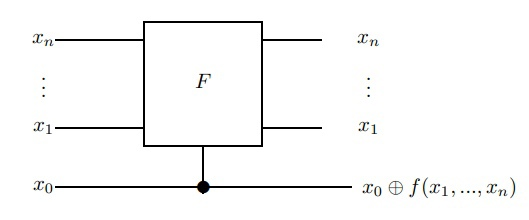
\includegraphics[scale=0.5]{img/aaa.jpg}}
	
	\label{nish}
\end{figure}


Тогда базис элементов из которых будут создаваться схемы представляет из себя:

% TODO заменить все вентили на элементы и все переменные на биты
\begin{itemize}
	\item Элемент отрицания;
	\item Элемент Тоффоли.
\end{itemize}

Элемент отрицания можно рассматривать как элемент Тоффоли от 1 переменной.

Пример обратимой схемы \ref{circuit_example1}

\begin{figure}[h]
	\caption{Пример обратимой схемы}
	\centering
	%Рамка только для изображений с белым фоном
	\fbox{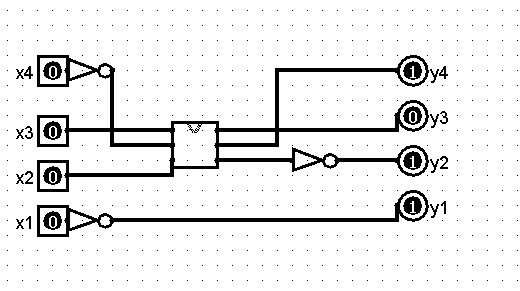
\includegraphics[scale=0.5]{img/circuit.jpg}}
	
	\label{circuit_example1}
\end{figure}
 
\mysubsubsection{Базис Тоффоли}
Базисом Тоффоли называется группа из схем, которые образовывают группу самых минимально возможных схем, например, схема, состоящая из 0 элементов, является минимальной, однако стоит заметить, что данная схема присутствует в любом наборе элементов и является основополагающей для создания схем, по этому она не учитывается.  В данном случае же образующие схемы будут состоять из следующих:

\begin{itemize}
	\item Элемент отрицания который инвертирует значение первого  бита присвоим обозначение 0;
	\item Элемент отрицания который инвертирует значение второго  бита присвоим обозначение 1;
	\item Элемент отрицания который инвертирует значение третьего  бита присвоим обозначение 2;
	\item Элемент отрицания который инвертирует значение четвёртого бита присвоим обозначение 3;
	\item Элемент Тоффоли который работает с первым, вторым и третьим битами присвоим обозначение 4;
	\item Элемент Тоффоли который работает с первым, вторым и четвёртым битами присвоим обозначение 5;
	\item Элемент Тоффоли Элемент Тоффоли который работает с первым, третьим и четвёртым битами присвоим обозначение 6;
	\item Элемент Тоффоли Элемент Тоффоли который работает с вторым, первым и третьим битами присвоим обозначение 7;
	\item Элемент Тоффоли Элемент Тоффоли который работает с вторым, первым и четвёртым битами присвоим обозначение 8;
	\item Элемент Тоффоли Элемент Тоффоли который работает с вторым, третьим и четвёртым битами присвоим обозначениее 9;
	\item Элемент Тоффоли Элемент Тоффоли который работает с третьим, первым и вторым битами присвоим обозначение 10;
	\item Элемент Тоффоли Элемент Тоффоли который работает с третьим, первым и четвёртым битами присвоим обозначение 11;
	\item Элемент Тоффоли Элемент Тоффоли который работает с третьим, вторым и четвёртым битами присвоим обозначение 12;
	\item Элемент Тоффоли Элемент Тоффоли который работает с четвёртым, вторым и третьим битами присвоим обозначение 13;
	\item Элемент Тоффоли Элемент Тоффоли который работает с четвёртым, первым и вторым битами присвоим обозначение 14;
	\item  Элемент Тоффоли Элемент Тоффоли который работает с четвёртым, первым и третьим битами присвоим обозначение 15.
\end{itemize}








 
%TODO СХЕМНО ПОКАЗАТЬ ФУНКЦИИ





%==============
\mysection{Методы минимизации обратимых схем}




%Добавить что-то что пояснить что минимизация это поиск


\mysubsection{Полный перебор}
К задаче полного перебора можно подойти двумя способами:
\begin{enumerate}
	\item Перебрать все возможные комбинации обратимых логических элементов;
	\item К схемам сложности $n-1$ добавлять схемы сложности 1 чтобы получить схемы сложности $n$.
\end{enumerate} 
Первый способ простой в реализации. Однако несмотря на простоту данного метода, потребуются крайне большие вычислительные затраты, ведь придётся перебрать $(16!)^{n}$ возможных вариантов, где $n$ --- максимальная сложность схемы, то есть $18\times 10^{427}$, при условии что $n=32$\cite{1201583}.
Второй же способ несколько сложнее, однако число комбинаций, которые необходимо будет проверить на порядки меньше чем при первом. Данный метод заключается в последовательном добавлении к некоторому множеству новые элементы к его концу. Например, пусть имеется схема, сложность которой равно 0, то есть функция не содержит никаких логически обратимых элементов, схему можно увидеть на рисунке \ref{circuit_0}.

\begin{figure}[h]
	\centering
	\caption{Схема сложности 0}
	%Рамка только для изображний с белым фоном
	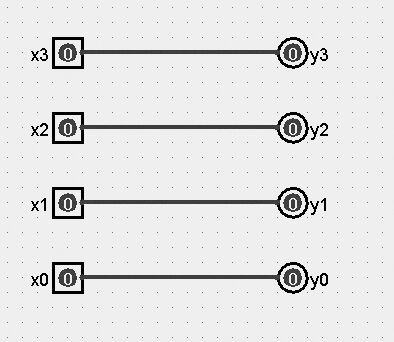
\includegraphics[scale=0.4]{img/simple.jpg}
	
	\label{circuit_0}
\end{figure}
 Такая функция всегда будет отправной точкой, так как она содержит в себе 0 элементов, и она существует всего одна, то есть это минимальная схема которая реализует функцию $(0, 1, 2, 3, 4, 5, 6, 7, 8, 9, 10, 11, 12, 13, 14,15)$. Теперь чтобы создать схему сложности 1, необходимо убрать выходы данной схемы и вместо них концы необходимых потоков совместить с началом элемента и получившейся схеме добавить выходы. Добавив к схеме элемент Тоффоли который работает на потоках $(0, 1, 2)$ получается схема вид которой можно увидеть на рисунке \ref{circuit_sup}.
 
 \begin{figure}[h]
 	\centering
 	\caption{Совмещённая схема}
 	%Рамка только для изображний с белым фоном
 	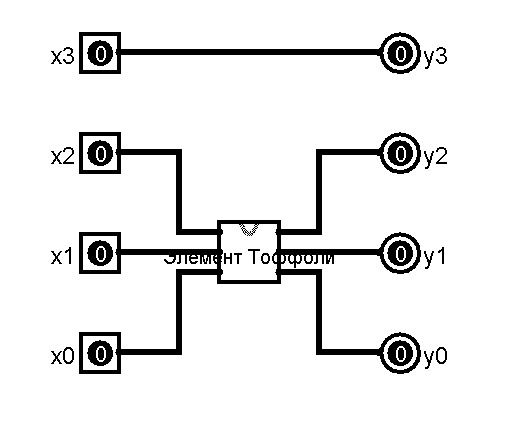
\includegraphics[scale=0.5]{img/added.jpg}
 	
 	\label{circuit_sup}
 \end{figure}
Так как схема собралась из схемы сложности 0 и элемента Тоффоли который работает на потоках $(0, 1, 2)$, то получилась не только минимальная схема, но и уникальная. Таким образом можно собрать все минимальные схемы во много раз быстрее и перебирая на множество порядков операций меньше, ведь чтобы получить схему сложности 4, нужно взять схему сложности 3 и добавить к ней какой-то элемент, однако с увеличением числа элементов, которые используются для реализации функции, могут начинать появляться схемы функции, которых уже реализованы, тогда их нужно где-то хранить и проверять есть ли у нас уже созданная такая функция.





%делать минус пять к страницам





\mysubsection{Библиотека минимальных схем}
Поскольку полное создание библиотеки минимальных схем задача невозможная, а использовать случайный перебор всех возможных комбинаций на таком большом пространстве решений ничем не лучше полного перебора, необходимо использовать некоторые другие подходы. Одним из таких подходов является поиск схемы сложности n путём соединения двух схем различной или одинаковой сложности. Тогда сложность итоговой схемы будет $n+m$, где n--- сложность схемы 1, m --- сложность схемы 2, при условии, что место соединения схем не имеет одинаковых элементов, иначе итоговая ложность схемы будет меньше, однако проблемой это является не будет, ибо схема всё ещё может дать правильное начальное положение.

  \begin{algorithm}
	\caption{Создание библиотеки}\label{alg:bib}
	\begin{algorithmic}[1]
		
		\Procedure{Library\_crt}{}
		\State $test\_dict=[\ldots]$ // коды элементов
		\State $circ\_list=[\ldots]$ // начальные комбинации
		\State $lib=library(4)$
		\Function{place\_and\_calculate}{$element\_list$}
		\State $lib.clear()$\par
		\State\algorithmicfor{ $element\_list !=0$}\par 
		\State\ldots
		
		\State \Return $lib.calculate()$
		\EndFunction
		\State
		\State\algorithmicfor{ $len(circ\_list[-1][-1]) <=6$}
		\State $circ\_list.append()$
		\State \algorithmicfor{ $len(circ\_list[-1][-1])$}\par
		\State\algorithmicfor{ $len(circ\_list[1])$}
		\EndProcedure
		
		
	\end{algorithmic}
\end{algorithm}




Соединения конца одной схемы с началом другой будем называть суперпозицией схем. %TODO
После соединения схем максимальная сложность схемы будет составлять $n+m$, где n --- сложность схемы 1, m --- сложность схемы 2. Однако в месте соединения схем могут стоять операции, которые аннулируют друг друга, например, два отрицания которые идут на одном потоке и аннулируют друг друга, вследствие чего их необходимо будет убрать. Пусть у нас есть две  схемы, представленные на рисунке \ref{circuit_65}:





\begin{figure}[h]
	\centering
		\caption{Пример схем сложности 6 и 5}
	%Рамка только для изображний с белым фоном
	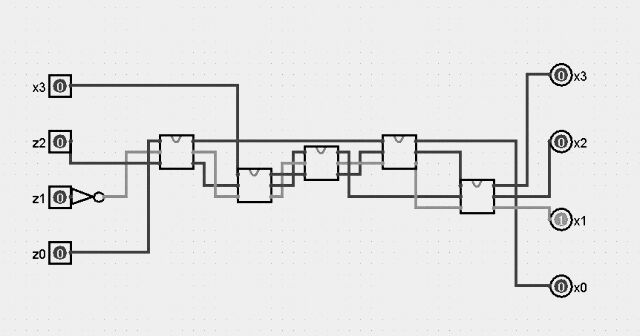
\includegraphics[scale=0.32]{img/first.jpg}
	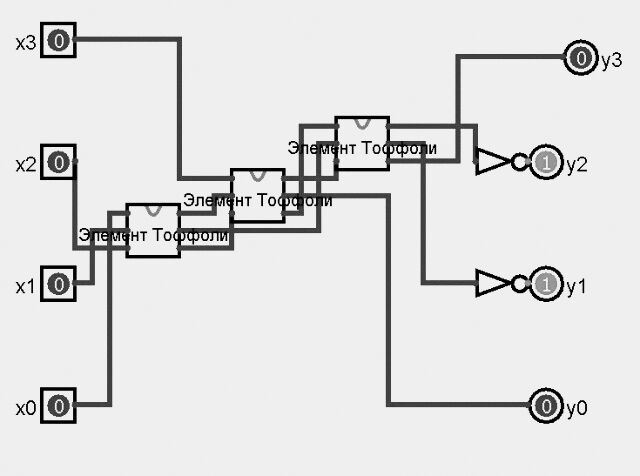
\includegraphics[scale=0.32]{img/second.jpg}

	\label{circuit_65}
\end{figure}

Данные схемы уже находятся в библиотеке поэтому они точно являются минимальными. Зная, что схемы являются минимальными можно попробовать составить из них схему некоторой размерности, то есть сделать суперпозицию схем. Однако достоверно узнать нельзя получится ли таким образом схема которая будет минимальной, если схема реализует уже некоторую функцию, которая есть в библиотеке, то тогда можно конечно сказать, что она будет не минимальной, но так как она уже есть в библиотеке, то она не принесёт никакой пользы в поисках нужной или схемы меньшей сложности. Результат совмещения схем можно увидеть на рисунке \ref{circuit_amal}.


\begin{figure}[h]
	\centering
	\caption{Пример суперпозиции схем}
	%Рамка только для изображний с белым фоном
	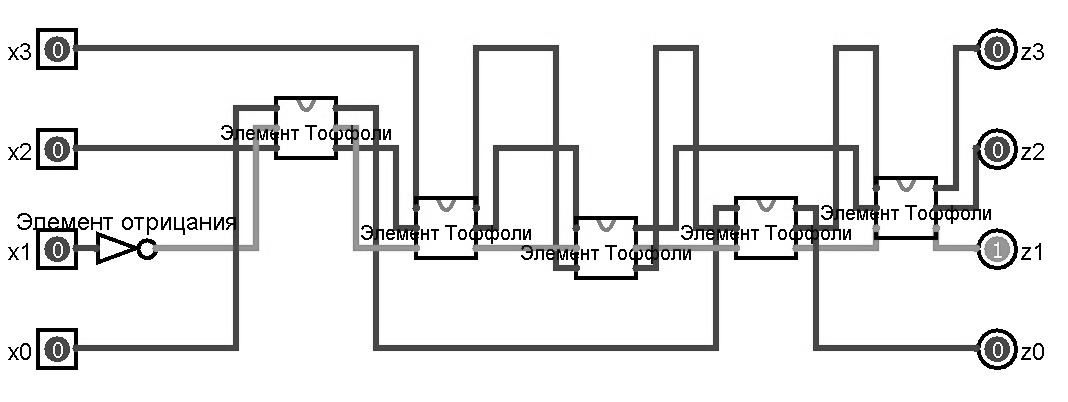
\includegraphics[scale=0.35]{img/amakgam.jpg}
	
	\label{circuit_amal}
\end{figure}

Схема, собранная из комбинации двух новых, реализует схему которой нету в библиотеке, соответственно её можно использовать как начало поиска минимальной схемы, так как сложность схемы составляет 11, то максимальную сложность схемы, которую стоит искать будет 10, на один элемент меньше, в зависимости от найденной схемы — это может достаточно сильно ускорить алгоритмы поиска.

Однако совмещение схем может привести к случаям, когда схема почти полностью или абсолютно сходится к какой-то простой. Схемы необходимые для примера можно увидеть на рисунке \ref{circuit_3}:


\begin{figure}[h]
	\centering
	\caption{Схемы сложности 3}
	%Рамка только для изображний с белым фоном
	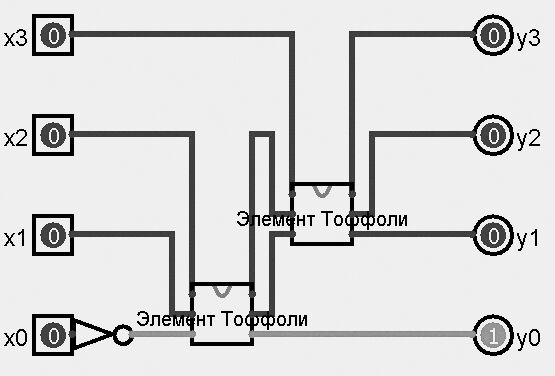
\includegraphics[scale=0.4]{img/test 1.jpg}
	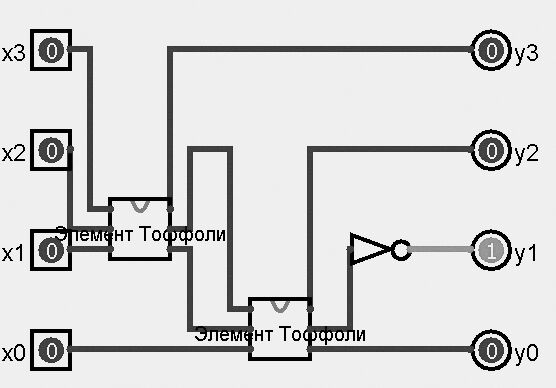
\includegraphics[scale=0.4]{img/test 2.jpg}
	
	\label{circuit_3}
\end{figure}

Данные схемы реализуют две различные пусть и похожие схемы, несмотря на их размерность они всё ещё могут дать схему размерности хотя бы 6 или немного меньше. Результат совмещения схем можно увидеть на рисунке   \ref{circuit_amal32} :


\begin{figure}[h]
	\centering
	\caption{Совмещённые схемы сложности 3}
	%Рамка только для изображний с белым фоном
	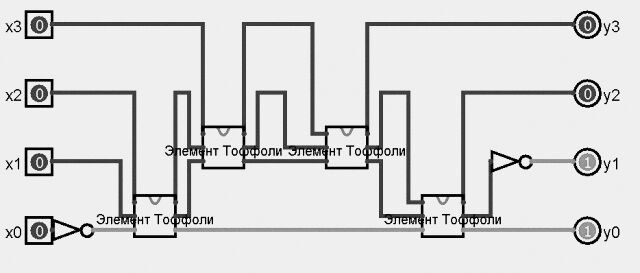
\includegraphics[scale=0.5]{img/modifed 2.jpg}
	\label{circuit_amal32}
\end{figure}
Такая схема может спокойно реализовать какую-то обратимую функцию, однако одинаковые элементы, стоящие рядом, друг с другом аннулируют друг друга, можно заметить, что тут только одна такая пара, однако если её убрать, то вторая пара элементов Тоффоли тоже должна быть убрана. Поиск комбинаций элементов которые аннулируют друг друга начинает особенно сильно проявляться при при поиске схем сложность которых близка к максимальной, ввиду числа позиций на которых могут стоять элементы. Конечный вид схемы представлен на рисунке \ref{circuit_amalW3}:


\begin{figure}[h]
	\centering
	\caption{Преобразованная схема}
	%Рамка только для изображний с белым фоном
	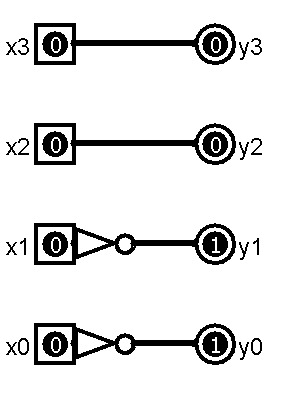
\includegraphics[scale=0.4]{img/cutted.jpg}
	\label{circuit_amalW3}
\end{figure}

Единственные элементы, которые остаются у данной схемы, это элементы отрицания, которые стоят на потоках 0 и 1, и поскольку производилась суперпозиция двух схем сложности 3, то скорей всего данная схема уже имеется, частое повторение полученных схем является одной из проблемы любого варианта создания библиотеки, однако даже если схемы построены так что элементы внутри них остаются, то всё ещё есть вероятность что такая схема реализует функцию, которая уже существует.

Алгоритм совмещения схем является средством поиска верхней границы сложности схем, выбирая случайную последовательность схем разных сложностей, поиск начинается от схем сложности 7, до схем сложности 32, которая является верхней границей сложности для множества элементов $(T_{1},T_{3})$, где $T_{1}$ --- элемент отрицания, $T_{3}$ --- элемент Тоффоли. Данный алгоритм является модифицированной версией алгоритма создания библиотеки, при создании которой добавляются базовые элементы к схеме меньшей сложности, в алгоритме совмещения же используются целые схемы, такой подход позволяет находить схемы быстрее чем если бы мы искали их случайно или расставили бы несколько ключевых точек в каждом уровне сложности.


  \begin{algorithm}
	\caption{Совмещение схем}\label{alg:bib}
	\begin{algorithmic}[1]
		
		\Procedure{circ\_fnd}{}
		\State $circ=[]$
		\State $pattern=[\ldots]$
		\State $lib=library(4)$
		\Function{remove\_pattern}{$circ\_list$}
		\For{ $i\  in range(0,len(circ\_list))$ }
		\State \ldots
		\EndFor
		\EndFunction
		\While
		\State $circ \leftarrow create()$
		\State $circ \leftarrow merge(circ)$
		\State $circ \leftarrow remove\_pattern(circ)$
		\EndWhile
		\EndProcedure
		
		
	\end{algorithmic}
\end{algorithm}

Скорость нахождения необходимой схемы при данной реализации зависит от количества вариантов которые будут проверяться за раз и так же от того, где схема находится, ведь схему сложности 12 будет найти легче, чем схему сложности 27, по мима числа вариантов на скорость так же влияет то, как сгенерировались схемы, ведь при случайной генерации можно оказаться очень близко например в 20 шагах, а может оказаться далеко например несколькими уровнями сложности выше.



Полный перебор всех схем от 4-х аргументов на данный момент является задачей не реализуемой. Создаваемая библиотека со схемами сложность которых доходит до 9 занимает 7 Гб, 6 из которых приходятся на схемы сложность которых составляет 9. Уже при переходе схем со сложности 8 к 9 можно заметить резкий скачок в занимаемой памяти. Однако для хранения необходимо выделить уже в 7 раз больше место, для хранения библиотеки со схемами сложности 10 включительно, необходимо 47 Гб памяти. Теоретически же полная библиотека которая будет содержать в себе все минимальные схемы, которые представляются парой вектор истинности и набор элементов, будет занимать место на жёстком диске 2,4 Тб - 3 Тб.













\mysubsection{Генетический алгоритм}



Генетический алгоритм используется в качестве способа ускоренного перебора возможных комбинаций, с целью найти такую комбинацию функциональных элементов, при которой схема выдаёт такой же вектор значений, но при меньшем количестве функциональных элементов. Так как сложность схемы заранее не известна, и зависит от того, схему какой сложности сможет создать алгоритм совмещения схем, то необходимо создать популяцию которая будет охватывать в худшем случае все размерности, иначе максимальная сложность схемы будет на 1 элемент меньше чем та сложность, которую нашёл алгоритм совмещения. Тогда популяция будет делиться на уровни, где каждый уровень обозначает количество элементов из которых состоит схема. Необходимо так же понимать что алгоритм не гарантирует того что мы получим ответ и не гарантирует что ответ будет минимальным связанно как с самим алгоритмом, так и с количеством возможных схем.

Первым шагом --- генетического алгоритма является создание начальной популяции где каждая особь создаётся независимо от другой, благодаря такому подходу охватывается часть пространства решений, которое так же, как и популяция поделена на несколько уровней, в зависимости от количества элементов которые необходимы для создания функции. Для создания начальной популяции необходимо случайным образом создать последовательность чисел, которые кодируют элементы, сложность функций будет идти от 7 до n-1, где n --- сложность схемы которая была создана алгоритмом совмещения. Так как библиотека схем создана до сложности 7, все схемы меньшей размерности уже созданы и поэтому не имеет практического смысла добавлять их в популяцию.\par
Второй шаг --- сортировка особей от лучших, к худшим. Это необходимо для того, чтобы: во-первых, найти  способные к конкуренции особи, которые будут ближе к тому значению которое нам необходимо, во-вторых благодаря сортировке особи чьи значения на\par
Третий шаг --- скрещивание, один из самых важных шагов данного алгоритма. Ввиду того, что лучшие особи могут никогда не достичь необходимого ответа, было принято решение что доминантные особи будут скрещиваться с случайной особью. Скрещивание двух конкретных особей так же должно опираться на цель, из-за этого необходимо разбить скрещивание на два случая, когда первый родитель даёт начальную часть генов потомку, и когда это делает второй родитель, вероятность между событиями $50\%$. Такой шаг необходим ведь не известно какая часть родителя и какой из них имел больший вклад в успех или провал потомка. Создав таким образом некоторую часть особей, остальные создаются случайным образом дабы сильнее покрыть область решений в поисках правильного ответа.\par
Четвёртый шаг --- мутация. Мутация шаг несколько опасный, однако необходимый, некоторые особи могут быть крайне похожи друг на друга в следствии чего вычисления их значения дадут одинаковые результаты, для этого каждая особь кроме нескольких первых имеют некоторый шанс мутировать, мутация изменяет случайный ген у особи на какой-либо другой, изменятся могут как один, так и два гена. Однако мутация может как приблизить к правильному ответу, так и отдалить от него из-за её случайности.\par

Каждая особь при данном алгоритме выглядит следующим образом\par
$[\underbrace{[0, 3, 9, 1]}_\text{Геном} , \underbrace{[11, 10, 13, 8, 15, 14, 9, 12, 3, 2, 5, 0, 7, 6, 1, 4]}_\text{Вектор истинности}, \underbrace{8}_\text{Соответствие}]$.\par
\noindent Созданную популяцию затем необходимо вычислить, дабы найти вектора истинности каждой особи. Как и для любой задачи минимизации в поиске минимальной схемы необходимо найти общий параметр который будет использоваться в качестве параметра сравнения, данную роль выполняет расстояние Хэмминга и с помощью него происходит определение и сортировка особей по тому, как близки они к целевой функции.

\begin{itemize}
	\item Геном --- является набором вентилей которые используются для создания вектора;
	
	\item Вектор истинности --- вектор который получается после после вычислений;
	\item  Соответствие --- насколько данная особь похожа на целевую функцию.
\end{itemize}
Основные функции, которые необходимы для реализации любого генетического алгоритма это: скрещивание, мутация, отбор.
	
Функция повторного создания популяции --- оставляет без изменения две лучшие особи каждого уровня, эти особи потом скрещиваются со случайно выбранной. Остальное место в популяции заполняются случайно созданными особями, последний шаг скрещивания --- это мутация.


Функция скрещивания --- берёт n-первых генов от первой особи и соединяет их с $m-n$ генами второй особи, где:m-длинна генома особи, n-случайное число в диапазоне от 1 до $m-1$. Скрещивание так же может произойти таким образом, что первые n-генов будут взяты от второй особи, а не от первой, вероятность такого $50\%$.



Функция мутации --- на вход получает всю популяцию, каждая особь может мутировать с некоторой вероятностью, так же с вероятностью $50\%$ особь может мутировать дважды.

%Генетический алгоритм реализован двумя различными способами дабы сравнить не только скорость их выполнения, но и так же возможные варианты получения ответа.
%Первый способ --- основывается на случайно создаваемой популяции без какой-либо подготовки, то есть, геном каждой особи это случайно сгенерированный вектор который представляет собой набор кодов вентилей.




 \begin{algorithm}[h]
	\caption{Генетический алгоритм}\label{alg:Examples_gen}
	\begin{algorithmic}[1]
		
		\Procedure{Genetic\_Alg}{$size,cicl,n,m$}
		
		
		\State $pop\_size=size$
		\State $cicr\_size=n$
		\State $target=m$
		\State $mutation\_chance=0.8$
		\State $cycles=cicl$
		\State $popul\leftarrow create\_popul(pop\_size,cicr\_size)$
		\State\algorithmicfor{ $i!=cycles$ \algorithmicdo \par
			$popul \leftarrow calculate(popul)$ \par
			$popul \leftarrow level\_sort(popul)$ \par
			$popul \leftarrow fitness(popul)$ \par
			$popul \leftarrow sorting(popul)$ \par
			$popul \leftarrow reprod(popul)$}
		\EndProcedure
		
		
	\end{algorithmic}
\end{algorithm}


Генетический алгоритм так же необходимо распараллелить, это обусловлено количеством вычислений и манипуляций, которые необходимо произвести над все популяцией. Слабым местом всех алгоритмов и программы создания библиотеки является функция вычисления вектора истинности, которая занимает достаточно много времени, так же из-за распараллеливания генетического алгоритма была необходима функция сортировки особей по сложности их набора элементов иначе, все особи собираются в одном месте. В свою же очередь особи будучи объединёнными в одном месте не способны будут размножаться и следовательно алгоритм не будет работать.
%АААААААААААААААААААААААААААААААААААААААААААААААААААААААААААААААААААААААААААААААААААААААААААААААААААААААААА



%Второй способ --- требует предварительного создания библиотеки до схем сложности 7. Теперь наша популяция будет составлять не только случайно сгенерированные особи, но и те которые являются комбинацией из нескольких минимальных схем которые мы уже знаем. Данный подход не гарантирует того, что схема полученная из комбинации нескольких будет уникальной или минимальной, однако он даёт дополнительную точность. 

\mysubsection{Алгоритм имитации отжига}
Алгоритм имитации отжига  относится к алгоритмам, основанным на имитации физических процессов, а именно охлаждении рабочего металла. В металле при этом уже выстроена некоторая кристаллическая решётка, но атомы всё ещё могут двигаться между ячейками этой самой решётки, при этом поскольку вся материя хочет попасть в состояние с минимальной потенциальной энергией, в алгоритме имитации отжига это так же используется то есть, если решение которое предлагает перейти в состояние в котором ответ будет больше чем тот, в котором мы находимся сейчас, то переход не произойдёт, благодаря этому вся система постепенно движется к точкам минимума. Сам же переход атомов так же зависит от температуры материала, где переход происходит с некоторой вероятностью и чем ниже температура, тем ниже эта самая вероятность.
В отличии от генетического алгоритма, так как атомы являются решениями в данном методе, то не нужно расставлять их по уровням, можно сделать $n$ различных решений которые будут все в одном месте, и они же уже сами по себе будут перемещаться по пространству решений в зависимости от случая. За раз атомы могут перемещаться только на один элемент в какую-то сторону, если они перемещаются вверх или вниз, то у них соотвественно или добавляется элемент или наоборот убирается. При перемещении вправо или влево между ячейками одного уровня у атома меняется последний элемент на 1 единицу в большую или меньшую сторону.




Первым шагом алгоритма имитации отжига следует создание некоторого набора решений, которые не зависимы друг от друга, так как решения нету необходимости делить на уровни, то создаются решения размерности от $7-n-1$ где $n$--- сложность схемы которая была найдена алгоритмом совмещения, без разделения на уровни сложно определить, как хорошо покрывается область решений, однако это позволяет исследовать её, не ограничиваясь как в генетическом алгоритме.\par
Вторым шагом является определения позиции атомов и соответственно их потенциальная энергия, так как все передвижения должны идти только из состояния большей потенциальной энергии в меньшее, то это достаточно важный шаг, ведь если атомы будут перемещаться случайным образом по области решений, то такой подход будем ничем не лучше полного перебора случайных последовательностей и последующего повторного движения куда-то.\par
Третьим шагом алгоритма является определение направления движения. Так как точно сказать в какую сторону необходимо двигаться нельзя, то атомы могут перейти в каждую из сторон с равной вероятностью, но только при условии, что в новом состоянии потенциальная энергия будет меньше. Однако, так как одним из параметра при перемещении является температура, которая даёт атому дополнительную энергию, у атома так же есть шанс в зависимости от температуры перейти в состояние, в котором потенциальная энергия будет больше. Такой шаг может помочь выбраться из локального минимума или решения, которое якобы является близким к тому, что мы ищем, но на самом деле никогда рядом с ним не будет.\par

  \begin{algorithm}[h]
	\caption{Алгоритм имитации отжига}\label{alg:Examples_ann}
	\begin{algorithmic}[1]
		
		\Procedure{Anneling}{$Temp, atom\_numb,target$}
		\State $test\_dict=[\ldots]$ // коды элементов
		\State $lib=library(4)$
		
		\State $final\_pos=[]$
		\State $atom\_lattice\leftarrow create\_lattice(atom\_numb)$
		\State\While{ $5<=Temp$}
		\State $atom\_lattice\leftarrow position(atom\_lattice,target,final\_pos)$
		\State $atom\_lattice\leftarrow movement(atom\_lattice)$
		\State $Temp-=0.5$
		\EndWhile
		
		
		\EndProcedure
	\end{algorithmic}
\end{algorithm}


Каждый же атом при таком алгоритме должен выглядеть следующим образом 
$[\underbrace{[14, 4, 12, 6, 9]}_\text{Вектор элементов}, \underbrace{[0, 1, 2, 15, 4, 11, 14, 13, 8, 9, 10, 7, 3, 12, 5, 6] }_\text{Вектор истинности}]$.\par
Так как атомы передвигаются не зависимо от предыдущих решений и не зависимо друг от друга в большинстве случаев, то хранить коэффициент близости не имеет большого смысла, а его повторное вычисление достаточно быстро. Единственный момент, когда атомы как-то взаимодействуют друг с другом это если атом, нашёл решение, которое уже занято каким-то другим, в таком случае он должен сразу же совершить переход в новое состояние не зависимо от его энергии.





Алгоритм имитации отжига получился не таким обширным как генетический из-за того, что атомы мало взаимодействуют друг с другом, кроме того, что проверяют не занята ли ячейка, которая является ответом каким-то другим атомом. Однако даже такого взаимодействия более чем достаточно для того чтобы атомы могли найти какое-то решение.





\mysubsection{Метод роя частиц}
Метод роя частиц --- в основе которого лежит роевой интеллект животных, например, птиц. Плюсом данного алгоритма при его использовании является то, что не требуется знать градиент функции, что для задачи минимизации схем которая не имеет как такового распределения является хорошим дополнением. Алгоритм роя частиц подобно муравьиному и пчелиному относится к классу алгоритмов роевых, то есть в основе его работы лежит роевой интеллект, однако в отличии от муравьиного алгоритма где используются феромоны для поиска богатых источников пищи, то в данном алгоритме частицы будут взаимодействовать друг с другом. Рой частиц основывается на нескольких правил:
\begin{enumerate}
	\item Частицы находятся на некотором расстоянии друг от друга, это делается для того чтобы они не столкнулись, и чтобы каждое решение в рое было уникальным, такой способ позволяет значительно повысить покрытие пространства решений благодаря чему каждая частица будет уникальна, чего, например, может не быть в генетическом алгоритме
	\item Частицы должны двигаться примерно в одном направлений, данный пункт реализован путём распределения частиц и написания отдельной формулы для скорости.
\end{enumerate}
Для скорости движения частиц необходимо написать отдельную формулу, формула должна удовлетворять нескольким требованиям для данной задачи:
\begin{enumerate}
	\item По мере приближения к решению очень важно чтобы частицы начали замедляться дабы покрыть большее пространство вокруг него
	\item Если же частицы нашли какую-то функцию которая достаточно похожа на ту, которую мы ищем, но ей не является они должны иметь возможно покинуть это место.
\end{enumerate}
На основании перечисленных выше критериев была создана следующая математическая формула $TT=S*0.8*P*\dfrac{D}{7}$.\par
Где: \begin{itemize}
	\item $S$ --- скорость;
	\item $P$ --- параметр, отвечающий за скачок из локального минимума;
	\item $D$ --- как близка данная функция к необходимому ответу.
\end{itemize}
Про параметр $P$ стоит так же сказать что его действие основывается на проверке последних 3 позиций которые посетила частица, если она все три итерации цикла находилась в неизменной точке, то при следующей попытке передвижения она переместиться из этого самого минимума. Двигаются точки в свою очередь по заданным направлениям, где первый раз направление выбирается случайно, а при нахождении места которая больше похожа на ответ частицы будут двигаться по направлению к ней.
\begin{itemize}
	\item Вверх --- частицам добавляется новый элемент со случайным значением;
	\item Вниз --- у частиц убирается последний элемент;
	\item Влево --- частицы двигающиеся налево последовательно уменьшают значения своих элементов, если последний достиг нуля, то отнимается единица у предпоследнего, и так далее; 
	\item Вправо --- частицы двигающиеся вправо последовательно увеличивают значения своих элементов, то есть если последний элемент достиг 15, то единица добавляется к предыдущему, и так далее.
\end{itemize}

Первым шагом алгоритма роя частиц, является создание начальных частиц, так же, как и в алгоритме имитации отжига, популяция создаётся случайным образом где у каждой особи представляет из себя схему сложности $7-n-1$, где n --- сложность схемы которая была найдена алгоритмом совмещения. Так же необходимо найти частицу, которая будет находится ближе всех к некоторому минимуму и сделать её точкой, к которой частицы будут стремиться и по пути к ней исследовать другие точки на подходящие решения. Так же сохраняются все точки, которые частицы посетили, одной из целей сохранения точек, чтобы определить застряла ли точка где-то или нет.\par
Второй шаг алгоритма --- это определения направления движения для частиц. Частицы в отличии от атомов двигаются по направлению к некоторой точке, в данном случае это точка которая имеет меньшую разницу с целевой функцией, однако частицы могут двигаться так же, как и атомы, то есть вверх, вниз, влево, вправо, сделано это для того чтобы частицы не случайно перебирали варианты решений пока как-то попадут в точку, а чтобы они целенаправленно двигались.
\par

\nocite{matplotlib}
\nocite{dec}
\nocite{class}
\nocite{list}
Третий шаг алгоритма --- это расчёт функции скорости, частицы двигаются с некоторой скоростью и при приближении к цели они замедляются. Сделано это для того чтобы проверить крайние точки у решения на потенциальную возможность того, что они будут являться так же решением, возможно минимальным, возможно такой же размерности что и то к которому они движутся, деление параметра близости на 7, используется как средство замедления, где 7 используется как точка перехода между решениями которые потенциально слишком далеки и теми, которые достаточно близко.

Частицы же в отличии от других алгоритмов должны содержать достаточно большое количество информации как о себе, так и о том для этого необходимо чтобы они выглядели следующим образом:
\begin{itemize}
	\item Вектор элементов --- вектор, содержащий в себе элементы, которые необходимы для создания схемы;
	\item Вектор истинности --- вектор который содержит в себе значения, которые были получены путём работы, схемы которая указана в векторе элементов;
	\item Коэффициент близости --- числовая величина по которой определяется сколько различных позиций между данным вектором и целевым;
	\item Глобальный минимум --- минимальная точка к которой будут двигаться частицы, и которая потенциально является решением;
	\item Локальный минимум --- минимальные позиции по которым прошла точка.
\end{itemize}
Всё это необходимо для взаимодействия между точками, ведь подобно стае птиц где одна заметила источник пищи, то вся стая полетит в направлении где можно её найти, аналогичная ситуация происходит в реализации алгоритма для поиска схем, если какая-то частица нашла точку которая достаточно близко находится к решению, то все частицы начнут двигаться в направлении к ней, по пути исследуя другие потенциальные решения.


  \begin{algorithm}
  	
	\caption{Алгоритм роя частиц}\label{alg:Examples_swar}
	\begin{algorithmic}[1]
		
		\Procedure{Particle\_swarm}{$size, particle\_numb,target$}
		\State $test\_dict=[\ldots]$ // коды элементов
		\State $lib=library(4)$
		
		\State
		\State $global\_minimum=[]$
		\State $swarm\leftarrow create\_swarm(size,particle\_numb)$
		\State\algorithmicfor{ $i!=400$}
		\State\algorithmicfor{ $i!=len(swarm)$}
		\State $swarm\leftarrow local\_min(swarm)$
		\State $swarm\leftarrow global\_min(swarm)$
		\State $swarm\leftarrow move\_swarm(swarm)$
		
		
		
		\EndProcedure
		
		
	\end{algorithmic}
\end{algorithm}



Алгоритм роя частиц строиться полностью на взаимодействии и общении частиц ведь частицы должны не только двигаться в направлении минимальной точки, они так же должны передавать информацию друг другу о точках, о том, кто как расположен и так же помнить какие точки они посетили.
%ААААААААААААААААААААААААААААААААААААААААААААААААААААААААААААААААААААААААААААААААААААААААААААААААААААААААААААА
%==========================
\mysection{Сравнительный анализ алгоритмов}



%\mysubsection{Реализация алгоритмов}

%Первый способ полного перебора нету практического смысла создавать из-за его простоты и из-за его крайней неэффективности.
%Второй же способ и последующую библиотеку смысл создать есть, ведь даже если не делать полный перебор она является хорошим началом для поиска и последующей минимизации схем путём ограничения сложности сверху и небольшим шансом найти лучший вариант.

















%Стоит обратить внимание так же на количество функций, которые задействованы в работе алгоритма имитации отжига, а именно то что их достаточно мало, что есть некоторая слабость алгоритма отсутствие качественного взаимодействия.







\nocite{diff}

\nocite{diff1}

\nocite{inproceedings}

%\mysubsection{Вычисления и анализ}




Для вычислений были вручную созданы схемы, которые не находятся в библиотеке, одна из них однозначно имеет минимальную схему, состоящую из 7 элементов, у остальных же схем элементы подбирались таким образом, чтобы они как можно меньше влияли на близлежащие к ним элементы, однако нельзя сказать наверняка какую минимальную сложности они имеют. Теоретически же сложности функций были 10 для второй и 16 для третьей. 


\mysubsubsection{Генетический алгоритм}

Генетический алгоритм без затруднений находит минимальную форму функции из 7 элементов во всех случаях. С функции, состоящей приблизительно из 11 элементов, начинаются некоторые проблемы, например, уменьшается вероятность нахождения правильного ответа и так же увеличивается время прохождения одной итерации, но в большинстве случаев ответ всё ещё находится в течении часа. Результаты работы алгоритма можно увидеть на рисунке \ref{gen}.
\begin{figure}[h]
	\centering
	\caption{Работа генетического алгоритма}
	%Рамка только для изображний с белым фоном
	\includegraphics[scale=0.7]{img/figure_1.png}
	\label{gen}
\end{figure}





Для схемы сложности 16 эффективность и вероятность нахождения решения снизились, единственным вариантом который был найден является схема сложности 20, маловероятно что алгоритм бы нашёл ещё какие-либо решения, ведь по мимо уменьшения сложности с каждым найденным решением размерность которого меньше чем найденное, так же уменьшается область решений, даже при таких колоссальных значениях. Искать схемы большей сложности, стоит помнить, что область решений с каждым новым элементом растёт в геометрической прогрессии и, например, найти схему сложности 29 будет практически невозможно просто из-за всех тех схем, которые идут перед ней.

\mysubsubsection{Алгоритм имитации отжига}
Алгоритм имитации отжига пусть и способен находить какие-то решения, но его эффективность падает сильнее чем у генетического. Конечно он не был далёк от истины и показал похвальные результаты на схемах сложности 7 и 10, но полноценно минимальную он не нашёл. Результаты работы алгоритма можно увидеть на рисунке \ref{ann}.

\begin{figure}[h]
	\centering
	\caption{Работа алгоритма имитации отжига}
	%Рамка только для изображний с белым фоном
	\includegraphics[scale=0.8]{img/figure_2.png}
	\label{ann}
\end{figure}

%Для схемы сложности 16 найденное решение достаточно далеки от минимальных, значения были найдены с разницей в 40 минут, при повторном же запуске решение скорей всего найдено не было.
%TODO что-то


В целом способен алгоритм вполне рабочий и способен находить некоторые решения, однако с эффективностью меньшей чем генетический. Однако в чём алгоритм имитации отжига выигрывает так это скорость, начальные точки решений во всех случаях были найдены быстрее чем у генетического. Возможно при использовании какого-то алгоритма который будет совмещать методы  поиска двух алгоритмов, будет меньше время поиска или будут найдены схемы меньшей сложности. Однако при реализации представленной в данной работе, алгоритм не способен гарантировать нахождение схемы меньшей сложности.

\mysubsubsection{Алгоритм роя частиц}

Алгоритм роя частиц показывает хорошие результаты, для схем сложностей 7 и 10 были найдены минимальные схемы. Конечно рой частиц несколько уступает генетическому, однако рой способен коллективно собираться в радиусе некоторых точек и рассматривать их область решений которая лежит непосредственно рядом с ними лучше, чем генетический или метод отжига. Результаты работы алгоритма можно увидеть на рисунке \ref{swarm}. 


\begin{figure}[h]
	\centering
	\caption{Работа алгоритма роя частиц}
	%Рамка только для изображний с белым фоном
	\includegraphics[scale=0.75]{img/figure_3.png}
	\label{swarm}
\end{figure}

Алгоритм роя частиц достаточно близко подходит к таким же результатам на схеме сложности 16, однако поскольку результаты сравнений проводились лишь на одной выборке сложно утверждать о достаточно схожей их эффективности, однако точно можно сказать что он опередил алгоритм имитации отжига.


\mysubsubsection{Сравнение трёх алгоритмов}

После сравнения алгоритмов самих с собой на схемах разной сложности, стоить сравнить все три, но только на одной какой-то схеме. Для такого была создана схема из 13 элементов, сложность схемы которая была найдена алгоритмом совмещения равна 25, каждый алгоритм работал в течении часа и было сделано три попытки для каждого алгоритма, из этих трёх выбиралась та, которая является лучшей. Сравнение работы алгоритмов можно увидеть на рисунке \ref{compare}.


\begin{figure}[h]
	\centering
	\caption{Сравнение алгоритмов}
	%Рамка только для изображний с белым фоном
	\includegraphics[scale=0.8]{img/figure_4.png}
	\label{compare}
\end{figure}

Пусть решения выбирались по тому какое было лучше, в данном случае выбиралось то решение которое могло найти минимум или что-то достаточно близкое к нему вне зависимости от того в какой временной промежуток оно было найдено, сколько решений было найдено перед этим, даже учитывая такие особенности проверки, алгоритм имитации отжига, достаточно сильно теряет свою эффективность при повышении сложности схемы. Генетический алгоритм и рой частиц же имеют достаточно хорошую эффективность и способны находить схемы приблизительной сложности 14-15.




Все расчёты и сравнения проводились на 8 ядерном процессоре с 16 потоками и тактовой частотой 3.2 ГГц.
%-------------
%Заключение 
%-------------
\mynonumbersection{ЗАКЛЮЧЕНИЕ}


Стандартные алгоритмы оптимизации являются достаточно хорошим инструментом для разного типа задач и здесь они оказались не исключением. Алгоритмы способны достаточно быстро находить результаты для схем средней сложности, а именно 11-15, однако, чем больше появляется схем которые необходимо проверить, тем мало эффективней становятся поиски. Даже если каждый алгоритм будет написан с распараллеливанием по  количеству потоков превышающее 20 возникает проблема того, что область решений увеличивается не пропорционально эффективности этих алгоритмов, а повышая количество потенциальных решений который один алгоритм способен проверять и соответственно вычислять, будет становиться всё больше и больше пока даже параллелизм не сможет повышать эффективность поиска решений и помогать в их нахождении, иными словами для схем больших сложностей, чем больше ресурсов будут потрачены на поиск решений, тем менее эффективными будут поиски решений, данная проблема затрагивает все алгоритмы не зависимо от того как они сделаны, ведь все алгоритмы работают в одной области решений, но она затрагивает каждый алгоритм по разному, генетический например такая проблема затронет сильнее при данной реализации из-за небольшого количества особей на одном уровне сложности, в то время как алгоритм отжига и рой частиц создаются сразу на всём множестве и могут свободно перемещаться по нему.


Генетический алгоритм --- основа этого алгоритма лежит в естественном отборе, количестве и мутациях особей. Данному алгоритму очень помогло то, что особи были разделены на уровни, взаимодействие особей, но даже при том числе особей, которые были созданы на каждом уровне, один цикл генетического алгоритма выполнялся медленнее, чем у роя частиц или имитации отжига. Взаимодействие особей достаточно важно ведь даже алгоритм совмещения схем строиться по принципу добавления нового элемента к существующей схеме. Генетический алгоритм несколько даже копирует поведения алгоритма совмещения, путём объединения двух схем от разных точек что так же помогает ему в нахождении ответа.  Стоит так же сказать, что на более высоких сложностях у схем, как бы особи не старались они не способны будут найти решение, несмотря на все мутации и случайное создание популяции, из-за того, что каждый дополнительный элемент увеличивает пространство решений в геометрической прогрессии, потребуется так же увеличивать количество особей в разы, что негативно скажется на производительности. Одним из возможных улучшений алгоритма может послужить увеличение числа позиций, на которых может происходить мутация, ведь увеличивая число элементов которые могут измениться также, увеличиваются и шансы нахождения нужной схемы или той, что близка к искомой.

Алгоритм роя частиц --- основа данного алгоритма лежит во взаимодействии некоторых групп животных, рыб или птиц, например, которые общаются между собой и передают информацию. Именно информация и взаимодействие между частицами помогли им добиться таких результатов, которые действительно способны противопоставляться генетическому алгоритму. Так же благодаря тому, что частицы имеют отдельную функцию для вычисления скорости они способны двигаться сообща и это помогло и дало возможность показать свою эффективность в нахождении схем. Однако алгоритм не без своих проблем, вполне возможно, что частицы будут достаточно часто находить решения, которые близки, но не являться решениями, и все частицы которые будут перемещаться в другие места будут продолжать возвращаться в эту самую точку из-за того, что область решений действительно большая отрицать такую возможность нельзя. 

Алгоритм имитации отжига --- основа работы данного алгоритма лежит исключительно в фундаментальных свойствах металлов. Алгоритм показал достаточно хорошие результаты для схем сложности близкой к той, на которой построена библиотека, однако схемы сложности 14 и более показывают то, что алгоритм справляется хуже тех, одна из причин — это отсутствие взаимодействия. Возможность обмениваться друг с другом решениями или информацией как таковой в такой задаче является как можно заметить крайне полезным качеством, именно поэтому генетический алгоритм и рой частиц имеют эффективность на средних сложностях выше. Так же размеры области решений и методы работы алгоритма не позволяют ему показать похожие результаты как остальные. Переход из меньшего состояния в большее это хорошая идея и на каких-то задачах она позволяет с уверенностью находить решения, однако, когда имеется столько решений, где малейшее отклонение может привести к точку не возврата, то эффективность алгоритма сильно зависит от того, какие параметры были заданны. Потенциальной идеей для модификации же может служить 

%Однако несмотря на всё выше сказанное так же нужно сказать следующее, универсальными эти алгоритмы далеко не являются, если они и способны найти минимальную форму схемы размерности, например, 13, они скорей всего не смогут найти минимальную форму схемы размерности 20 и выше. 
Плюсом всех алгоритмов минимизации же который не один раз использовался в данной работе, это возможность их модифицировать, добавляя некоторые особенности, например разделение на уровни, отталкивание одинаковых решений, понижение сложности при нахождении решения. Алгоритму роя частиц, например можно добавить что-то похожее на операцию скрещивания в генетическом алгоритме, которая например будет брать три случайные частицы, с помощью триангуляции находить место которая является серединой между этими тремя и отправлять частицу в вычисленную позицию. Алгоритм имитации отжига же может взять например идею того, что атомы будут держаться на некотором расстоянии друг от друга и взависимости  от температуры это расстояние будет увеличиваться что позволит атомам покрыть пространство несколько большее, однако с температурами близкими к минимуму расстояние между ними может быть достаточно велико чтобы один атом например отталкивал другие от решения, в которое он сам не попадёт.
Проблема поиска минимальной схемы и эффективность алгоритмов поиска, тесно связан с тем, какой сложности схему необходимо найти, ведь схема сложности 20 может иметь за собой несколько сотен миллиардов не только схем размерности 20, но и так же схемы меньшей размерности, в то время как схемы сложности 14 могут иметь количество меньше 10 миллиардов, Ведь каждый дополнительный элемент не только даёт возможность схеме реализовать новые, но и добавляет новую форму для старых схем, и в какой-то момент число схем которые реализуют уже существующие функции становится много больше чем те, которые добавляются, особенно сильно такое будет заметно на сложностях близки к максимальным, данное свойство всегда будет являться проблемой для задачи поиска минимального вида схемы. Даже при всех особенностях алгоритмов и  теоретической выгоде которая последует из их объединения, маловероятно что с помощью неё получится что-то, что будет способно гарантированно находить минимальные схемы любой сложности и это, не говоря о схемах, которые имеют 5 входов и более.


%В результате выполнения дипломной работы были получены следующие результаты:
%Наблюдением и потенциальным направлением для оптимизации подобных схем является искусственный интеллект. Достаточно обученный и способный к анализу искусственный интеллект теоретически будет способен создавать схемы случайной размерности и последовательно их минимизировать, ведь обратимые операции, являются ничем более как перестановкой значений на некоторых позициях, как например элемент Тоффоли размерность которого равно количеству входов схемы является ничем более как транспозицией двух рядом стоящих выходных значений.

На основе проведённых исследований можно сделать ещё один вывод. Из-за того, что каждая схема имеет уникальное строение, которое воссоздать методами стандартной минимизации как те что представлены в данной работе будет достаточно сложно для схем сложности 5. Однако, по вектору истинности можно проследить некоторые закономерности в расстановке логически обратимых элементов и благодаря этой самой закономерности теоретически можно будет обучить искусственный интеллект, который будет анализировать и составлять схемы некоторой размерности с большей эффективностью чем алгоритмы минимизации. Благодаря как раз поиску закономерностей и знанию того как каждый элемент работает искусственный интеллект теоретически сможет составлять схемы с 4 входами и потенциально при достаточном наборе обучающих данных будет способен создавать схемы сложности пять и более.   %Ещё одним потенциальным направлением для улучшения в поиске минимальных схем будет использование алгоритмов которые сильнее зависят от других решений, как например пчелиный или муравьиные алгоритмы,
\nocite{10.5555/522098}

\nocite{488968}
\nocite{article}
\nocite{brownlee-clever-algorithms-nature-2011}
\nocite{diff1}
\nocite{inproceedings}



%-------------
%Список литературы
%-------------
\newpage
%Для включения в диплом списка литературы подключается файл literature.bib
%В нем приведены наиболее часто встречающиеся типы библиографических ссылок
\renewcommand{\refname}{СПИСОК ИСПОЛЬЗОВАННЫХ ИСТОЧНИКОВ}
\addcontentsline{toc}{section}{\refname}
\printbibliography
%-------------
%Приложения
%-------------

\addappendix{Классы элементов}

\begin{lstlisting}[language=Python, caption={Класс реализующий вентиль отрицания}, label=Not_gate]
	class Not_Gate:
	def __init__(self, lain): self.lain=lain
	def use_Not(self,num): return num ^ (1 << self.lain)
	def __str__(self): return "Npt on lain: {}".format(self.lain)
	
\end{lstlisting}

\begin{lstlisting}[language=Python, caption={Класс реализующий вентиль Тоффоли}, label=Toffoly]
	class Toffoli_Gate:
	def __init__(self,lains): self.lains=lains
	
	def use_Toffoli(self,num):
	binar = bin(num)[2:].zfill(4)
	binar = list(map(int, binar))
	binar[self.lains[0]] = binar[self.lains[0]] ^ (binar[self.lains[1]] & binar[self.lains[2]])
	return int(''.join(list(map(str, binar))), 2)
	
	def __str__(self): return "Toffoly on lains: {}".format(self.lains)
	
\end{lstlisting}

\addappendix{Функции генетического алгоритма}



\begin{lstlisting}[language=Python, caption={Функция повторного создания популяции }, label=repopulate]
	def repopulate(pop):
	    new_pop=[[] for i in range(0,len(pop))]
	    new_pop[0]=pop[0]
	    for i in range(1,len(pop)):
	        for z in range(0,100):
	            new_pop[i].append([take_genes(pop[i][0][0],pop[i][rd.randint(1,len(pop[i])-1)][0])])
	        for z in range(0,pop_size-100):
	            new_pop[i].append(random_gates(len(pop[i][0][0])))
	    new_pop=mutation(new_pop)
	return new_pop
\end{lstlisting}


\begin{lstlisting}[language=Python, caption={Функция скрещивания }, label=take_genes]
	def take_genes(sub1,sub2):
	    child=[]
	    size=rd.randint(1,len(sub2)-1)
	    if rd.randint(1,2)==1:
	        for i in range(0, size):
	            child.append(sub1[i])
	        for z in range(i, len(sub2) - 1):
	            child.append(sub2[z])
    	else:
	        for i in range(0, size):
	            child.append(sub2[i])
	        for z in range(i, len(sub2) - 1):
	            child.append(sub1[z])
	    return child
\end{lstlisting}

\addappendix{Функции алгоритма   имитации отжига }

\begin{lstlisting}[language=Python, caption={Функция перемещения атомов}, label=take_genes]
def atom_movement(popul):
    new_move=[]
    for i in range(0, len(popul)):
        new_move=popul[i].copy()
        if checker(popul[i]): continue
        chance = rd.random()
        movement_chance = rd.random() * temperature
        if movement_chance>=0.25:
            if 0<chance<0.25:
                if len(popul[i][0]) == 0: continue
                pos=rd.randint(0, len(popul[i][0]) - 1)
                new_move[0][pos]=(rd.randint(0, popul[i][0][pos]))
            elif 0.25<=chance<0.5:
                new_move[0].append(rd.randint(0, 15))
            elif 0.5<=chance<0.75:
                if len(popul[i][0])==0: continue
                pos = rd.randint(0, len(popul[i][0]) - 1)
                new_move[0][pos] = \
                    (rd.randint(popul[i][0][pos], 15))
            elif 0.75<=chance<1:
                if len(popul[i][0]) == 0: continue
                new_move[0].pop()
        new_move[2]=entropy_check(new_move[1],target)
        #print(new_move[2], popul[i][2])
        if new_move[2]<popul[i][2]:
            print(new_move,popul[i])
            popul[i]=new_move
\end{lstlisting}



\addappendix{Функции роя частиц}


\begin{lstlisting}[language=Python, caption={Функция поиска глобального минимума }, label=take_genes]
def the_hunt(entire_swarm):
    min_min=18
    min_pos=-1
    for i in range(0,len(entire_swarm)):
        if min_min>entire_swarm[i].particle_postition:
            min_min=entire_swarm[i].particle_postition
            min_pos=i
    for z in range(0,len(entire_swarm)):entire_swarm[z]
    .global_minimum
    =[entire_swarm[min_pos].particle_body,entire_swarm[min_pos]
    .particle_postition]

\end{lstlisting}

\begin{lstlisting}[language=Python, caption={Функция добавления-убавления позиций}, label=take_genes]
def add_remove(body_list,number,oper):
    if oper==1:# минус
        while(number!=0):
            number-=1
            if body_list[-1]-1==-1:
                for i in range(1,len(body_list)+1):
                    if body_list[-i]==0:
                        body_list[-i]=15
                    else:
                        body_list[-i]-=1
                        break
            else: body_list[-1]-=1
    elif oper==2:
        while(number!=0):
            number-=1
            if body_list[-1]+1==16:
                for i in range(1,len(body_list)+1):
                    if body_list[-i]==15:
                        body_list[-i]=0
                    else:
                        body_list[-i]+=1
                        break
            else: body_list[-1]+=1
    if all_equal(body_list)==True:
        return random_creator_sized(len(body_list))
    return body_list

\end{lstlisting}







\begin{lstlisting}[language=Python, caption={Функция вычисления вектора истинности }, label=take_genes]
def placer_and_calculator(diff_element):
    lib.clear()
    for i in range(0, len(diff_element)):
        if 0 <= diff_element[i] <= 3:
            lib.place_Not(test_dict[str(diff_element[i])])
        else:
            lib.place_Toffoli(test_dict[str(diff_element[i])])

    arrr = [i for i in range(0, 16)]

    for j in arrr: arrr[j] = lib.calculate(j)
    return arrr

\end{lstlisting}
\end{document}

